% HFUT_Courge_Project
\documentclass[UTF8]{ctexart}
\usepackage{fancyhdr}
\usepackage{graphicx}
\usepackage[colorlinks,linkcolor=black]{hyperref} % [colorlinks,linkcolor=blue]
\usepackage{csvsimple}
\usepackage{titlesec}
\usepackage{titletoc}
\usepackage{booktabs}
\usepackage{listings}
\usepackage{appendix}

\usepackage{tabularx}
\usepackage{array}
\usepackage{bm, amsmath,amsfonts}
\usepackage{pdfpages}
\usepackage{multirow}
\usepackage[a4paper,left=3.4cm,right=3cm,top=1.65cm,bottom=2.54cm]{geometry}
\renewcommand{\contentsname}{\zihao{3} 目\quad 录}
\renewcommand{\abstractname}{\zihao{3} 摘\quad 要}
%页眉页脚设置
\pagestyle{fancy}
\fancyhf{}
\cfoot{\thepage}
\rhead{\kaishu~商务数据模拟分析~}

%目录页设置
\titlecontents{section}[0em]{\zihao{4}\bf }{\thecontentslabel\ }{}
{\hspace{.5em}\titlerule*[4pt]{$\cdot$}\contentspage}
\titlecontents{subsection}[2em]{\vspace{0.1\baselineskip}\zihao{-4}}{\thecontentslabel\ }{}
{\hspace{.5em}\titlerule*[4pt]{$\cdot$}\contentspage}
\titlecontents{subsubsection}[4em]{\vspace{0.1\baselineskip}\zihao{-4}}{\thecontentslabel\ }{}
{\hspace{.5em}\titlerule*[4pt]{$\cdot$}\contentspage}
%代码设置
\RequirePackage{listings}
\RequirePackage{xcolor}
\definecolor{dkgreen}{rgb}{0,0.6,0}
\definecolor{gray}{rgb}{0.5,0.5,0.5}
\definecolor{mauve}{rgb}{0.58,0,0.82}
\lstset{
	numbers=left,  
	frame=tb,
	aboveskip=3mm,
	belowskip=3mm,
	showstringspaces=false,
	columns=flexible,
	framerule=1pt,
	rulecolor=\color{gray!35},
	backgroundcolor=\color{gray!5},
	basicstyle={\ttfamily},
	numberstyle=\tiny\color{gray},
	keywordstyle=\color{blue},
	commentstyle=\color{dkgreen},
	stringstyle=\color{mauve},
	breaklines=true,
	breakatwhitespace=true,
	tabsize=3,
}
%------------------------------------------------------------------------
%正文部分
\begin{document}
	\begin{titlepage}
		\centering
		\vspace*{1cm}
		\quad
\includegraphics[width=10.53cm]{HIT.jpg}\\
		\vspace*{0.5cm}
		{\fontsize{60pt}\baselineskip 研\qquad\ 究\qquad\ 报\qquad\ 告}
		 \vskip 7cm
		 \fontsize{13pt}\baselineskip
		 \makebox[20mm]{报告题目}
		 \underline{\makebox[95mm][c]{XXXXXX}}\\%在这里修改成自己的题目
		 \vskip 0.9cm
		 \makebox[20mm]{学生姓名}
		 \underline{\makebox[95mm][c]{XXXXXX}}\\
		 \vskip 0.9cm
		 %\makebox[40mm]{学\qquad\qquad 号}
		 %\underline{\makebox[75mm][c]{ \LARGE 1183300114}}\\
		 %\vskip 0.9cm
		 \makebox[20mm]{学号}
		 \underline{\makebox[95mm][c]{XXXXXXX}}\\
		 \vskip 0.9cm
		  \makebox[20mm]{授课教师}
		 \underline{\makebox[95mm][c]{XXXXXXX}}\\
		 \vskip 2cm
		 \LARGE \textbf{\number \year }~年~\textbf{\number\month}~月~\textbf{\number\day}~日		 
	\end{titlepage}

%\begin{abstract}
 %	\pagestyle{plain}
 %	\thispagestyle{empty}
 %	\zihao{-4}
%	\par 这是
%	\par 这是测
%	\textbf{关键字}:\quad 关键字 \quad 关键字 \quad 关键字 \quad 关键字
%	\newpage
%\end{abstract}

\tableofcontents\thispagestyle{empty}
\newpage
\setcounter{page}{1}
\section{研究背景}




如今,无论是对银行还是借款人来说,银行贷款都存在着诸多风险。银行贷款的风险分析需要对贷款的风险和风险水平有一定的了解,银行需要分析他们的客户的贷款资格,以便他们可以专门针对这些客户。

信贷风险的评估理论诸多,但是在面临已知的不同数据时,可操作性上一直存在诸多难题,而信贷是属于商业银行的一个核心利益点,商业银行也影响着整个金融行业,因此,信贷风险的评估会影响银行的信贷控制,一定程度上影响整个金融业,甚至国民经济走向。近年来,随着全球经济下行,中国经济增速放缓,信贷资金的评估控制日益得到关注,如何依据信贷风险等因素来确定是否放贷及贷款额度、利率和期限以及合理地控制和化解风险成为了一个重要的课题。

在实际中,由于个人体量相对很小,也缺乏抵押资产,但个人贷款仍然占据着市场中的许多份额,银行希望根据在线申请表中提供的客户详细信息,如性别、婚姻状况、年龄、职业、收入、债务等,实现贷款资格流程(实时)的自动化。随着银行业交易数量的快速增长和海量的数据量,可以方便地分析客户的行为,降低贷款风险。因此,根据银行的数据预测贷款类型和贷款额是非常重要的。



\section{数据准备}

本研究针对个人信贷问题,选取数据集来描述客户贷款数据,大约有100多个不同的客户详细信息样本,每个客户都在不同的行中表示。数据包含表\ref{tab:addlabel}中的示例但不限于这些内容。

数据中有包括ID、所在州、性别、年龄、种族、婚配、职业、信用卡分数、收入、月信用负债、贷款类型、贷款决策类型(放贷与否)信息。


% Table generated by Excel2LaTeX from sheet 'Sheet1'
\begin{table}[htbp]
	\centering
	\caption{Part Data }
	\vspace{0.3cm}
	\begin{tabular}{ccccccc}
		\toprule[1.5pt]
		ApplicantId & State & Gender & Age & Race  & Marital\_status & Occupation \\
		\midrule[1.0pt]
		004NZMX60E & CA    & Male  & 36    & No co-applicant & Married & NYPD \\
		004NZMX60E & CA    & Male  & 36    & No co-applicant & Married & NYPD \\
		017STAOLDV & OH    & Female & 34    & White & Married & IT \\
		017WEFEN7S & OH    & Male  & 48    & No co-applicant & Married & Accout \\
		01FSKXYCRD & FL    & Male  & 32    & White & Single & Business \\
		\bottomrule[1.5pt]
	\end{tabular}%
	\label{tab:addlabel}%
\end{table}%

\section{贷款流程自动化模型建立流程}
\subsection{导入数据并检查NA值}
首先将所有数据导入Rstudio中,并检查数据中是否有空值,如果有,则需要对空值进行处理。



\subsection{计算DTI}

DTI全称Debt to Income Ratios(通常缩写为DTI),是反映贷款者还贷能力的重要工具,将给居民的信贷消费带来巨大影响。IDT比率是消费者每月支付的总收入的百分比。(确切地说,DTI经常覆盖的不仅仅是债务,它们还可以包括本金、税金、费用和保险费。)

\begin{equation}
	DTI = \frac{Debts}{Income} *100
\end{equation}

\subsection{创建贷款决定状态变量}

贷款决定变量是我们用于贷款预测的目标变量,因为我们获得的数据中一级有贷款决策,所以我们将其处理为一个0-1变量,0代表Denied。

\subsection{选择预测所需的字段}

将将目标变量编码为factor后,我们需要选择贷款决定转状态变量为我们需要预测的字段。

\subsection{将分类变量编码为因子}

进一步,我们将分类变量编码为因子,分别将变量Gender转换为(1,2),其中1代表男性,2代表女性;将变量Marital\_status转换为(1,2,3),分别代表离异、结婚、单身三种状态;将变量Occupation转换成(1,2,3,4,5),分别代表会计、商业、IT、管理、警察;将变量贷款方式转换为(1,2,3,4),分别代表汽车信贷、行用卡、住房信贷、个人信贷。


\subsection{拆分集合}

将重新定义的客户数据集拆分为训练集和测试集,设置随机种子,按70\%为训练集,30\%为测试集进行拆分。

\subsection{数据处理}

在我们做数据的时候,一个数据会有很多特征;比如在描述影响房价的因素,有房子面积,房间数量等。而不同的特征存在不同的量纲,为了消除量纲、数值差异等,我们就需要对数据进行中心化和标准化,其计算方法为:

\begin{equation}
	Z = \frac{X-\bar{X}}{S}
\end{equation}
$S$为样本标准差,$X$为样本数值,$\bar{X}$ 为样本均值。

主成分分析,应用PCA对训练集和测试集进行降维。
\begin{equation}
	F_p = a_1i*Z_x1+a_2i*Z_x2+......+a_pi*Z_xp
\end{equation}
其中$a_1i, a_2i, ...,a_pi(i=1,...,m)$为X的协方差阵Σ的特征值所对应的特征向量,$Z_x1, Z_x2, ..., Z_xp$是原始变量经过标准化处理的值,因为在实际应用中,往往存在指标的量纲不同,所以在计算之前须先消除量纲的影响,而将原始数据标准化。



应用朴素贝叶斯分类模型预测贷款:

给定训练数据集$T = {(x_1,y_1),...,(x_n,y_n)}$ ,由$P(X,Y)$独立同分布产生,要得到该联合分布,需估计:

\begin{itemize}
	\item 先验 (prior) 概率分布
	\begin{equation}
		P(Y=c_k),k =1,2,...,K
	\end{equation}
	\item 条件概率分布
	\begin{equation}
		P(X=x|Y=c_k) = P(X^{(1)} = x^{(1)},...,X^{(n)} = x^{(n)})
	\end{equation}
	
\end{itemize}

应用贝叶斯定理:

\begin{equation}
	P(Y=c_k|X=x) = \frac{P(X=x|Y=c_k)P(Y=c_k)}{\sum_{k}P(X=x|Y=c_k)P(Y=c_k)}
\end{equation}

由此可预测数据标签:

\begin{equation}
	y = arg  \underset{c_k}{max} P(Y=c_k)\prod_{j}P(X^{J}=x^{(j)}|Y=c_k)
\end{equation}

随后预测测试集的结果并计算精度。
\section{结果}

\subsection{预测结果}
用测试集进行检验,使用混淆矩阵计算精度,我们可以看到,由于数据量不是非常充分,测试集结果仍存在较大偏差。

\begin{table}[h!]
	\centering
	\caption{PRED}
	\vspace{0.3cm}
	\begin{tabular}{ccc}
		\toprule[1.5pt]
		- & 0 & 1  \\
		\midrule[1pt]
		0  & 3   & 7  \\
		1  & 3   & 22 \\
		\bottomrule[1.5pt]
	\end{tabular}%
	\label{tab:a111}%
\end{table}%

\subsection{使用测试集的实际观察结果和预测结果绘制图}
从测试集取$min-1$和$max+1$值,构建网格,使用测试集的实际观察结果和预测结果绘制图如下:

其中红绿分割线为拟合后得到曲线,红色意味着在此区域的人不应获得贷款,而绿色可以获得。红绿的点分别是测试集中贷款决策分别为0和1的点,我们看到由于数据量较小,并不是所在区域的点为同一状态。
\begin{figure}[t!]
	\centering
	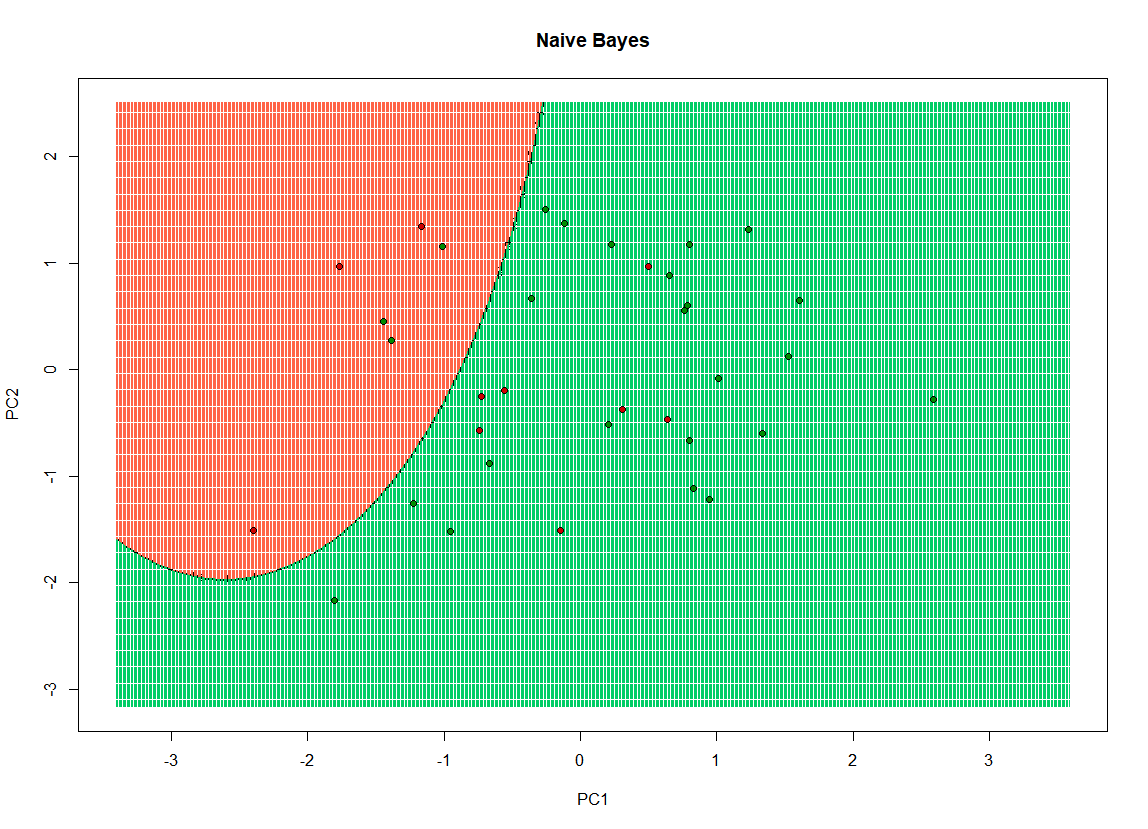
\includegraphics[width=0.8\linewidth]{Rplot.png}
	\caption{结果展示}
\end{figure}



\newpage
\newpage
\clearpage
\begin{appendices}

\section{代码}
\begin{lstlisting}[language=R]
rm(list=ls())
#--------------------------------------------------------------------------
library(lattice)
library(ggplot2)
customer_loan_details <- read.csv("C:/Users/10793/Desktop/cutomer_loan_details.csv", sep = ",")

#library(xlsx)
#write.xlsx(customer_loan_details,'1.xlsx')
# Print the structure of the dataframe
str(customer_loan_details)
head(customer_loan_details)

# Check for the NA values
any(is.na(customer_loan_details))

# Calculating DTI
customer_loan_details$dti <- (customer_loan_details$debts/customer_loan_details$income)*100

# Create loan_decision_status variable which is our target variable to use for loan prediction
customer_loan_details$loan_decision_status <- ifelse(customer_loan_details$loan_decision_type == 'Denied', 0, 1)

# Encoding the target variable as factor
customer_loan_details$loan_decision_status <- factor(customer_loan_details$loan_decision_status, levels = c(0, 1))

#Selecting the required fields for prediction
customer_loan_refined <- customer_loan_details[,c(3,4,6:8,11,13:14)]
head(customer_loan_refined)

# Encoding the categorical variable as factors
customer_loan_refined$gender <- as.numeric(factor(customer_loan_refined$gender,
levels = c('Male','Female'),
labels = c(1,2)))

customer_loan_refined$marital_status <- as.numeric(factor(customer_loan_refined$marital_status,
levels = c('Divorced','Married','Single'),
labels = c(1,2,3)))

customer_loan_refined$occupation <- as.numeric(factor(customer_loan_refined$occupation,
levels = c('Accout','Business','IT','Manager','NYPD'),
labels = c(1,2,3,4,5)))

customer_loan_refined$loan_type <- as.numeric(factor(customer_loan_refined$loan_type,
levels = c('Auto','Credit','Home','Personal'),
labels = c(1,2,3,4)))

head(customer_loan_refined)
#--------------------------------------------------------------------------
# Splitting the customer_loan_refined dataset into training and test sets
library(caTools)
set.seed(123)
split = sample.split(customer_loan_refined$loan_decision_status, SplitRatio = 0.70)
training_set = subset(customer_loan_refined, split == TRUE)
test_set = subset(customer_loan_refined, split == FALSE)
#--------------------------------------------------------------------------
#Applying Feature Scaling
training_set[-8] = scale(training_set[-8])
test_set[-8] = scale(test_set[-8])

head(training_set)

# Applying Dimensionality reduction using PCA to training and test sets
# install.packages("caret")

library(caret)
pca = preProcess(x = training_set[-8], method = 'pca', pcaComp = 2)
training_set_pca = predict(pca, training_set)
training_set_pca = training_set_pca[c(2, 3, 1)]
test_set_pca = predict(pca, test_set)
test_set_pca = test_set_pca[c(2, 3, 1)]
head(test_set_pca)

# Appling Naive Bayes classification model to predict the loan
# install.packages("e1071")
library(e1071)
classifier = naiveBayes(x = training_set_pca[-3], y = training_set_pca$loan_decision_status)

# Predicting the Test set results
y_pred = predict(classifier, newdata = test_set_pca[-3])

# confusionMatrix to calculate accuracy
confusionMatrix(table(test_set_pca[, 3], y_pred))
#--------------------------------------------------------------------------
# Visualising the Test set results
#install.packages("ElemStatLearn")  package ‘ElemStatLearn’ is not available (for R version 3.6.3)
#安装方法如下

#packageurl <- "https://cran.r-project.org/src/contrib/Archive/
#ElemStatLearn/ElemStatLearn_2015.6.26.tar.gz" ##这块复制上去
#install.packages(packageurl, repos=NULL, type="source")
library(ElemStatLearn)
set = test_set_pca

# Built the grid using X1, X2 by taking min-1 and max+1 values from test set
X1 = seq(min(set[, 1]) - 1, max(set[, 1]) + 1, by = 0.01)
X2 = seq(min(set[, 2]) - 1, max(set[, 2]) + 1, by = 0.01)
grid_set = expand.grid(X1, X2)
colnames(grid_set) = c('PC1', 'PC2')

# Predict the test set observations 
y_grid = predict(classifier, newdata = grid_set)

# Plot the graph using actual observations from test set and predicted results
plot(set[, -3], main = 'Naive Bayes',
xlab = 'PC1', ylab = 'PC2',
xlim = range(X1), ylim = range(X2))
contour(X1, X2, matrix(as.numeric(y_grid), length(X1), length(X2)), add = TRUE)
points(grid_set, pch = '.', col = ifelse(y_grid == 1, 'springgreen3', 'tomato'))
points(set, pch = 21, bg = ifelse(set[, 3] == 1, 'green4', 'red3')) 
\end{lstlisting}


\end{appendices}
	
\end{document}